\section{Ілюстрація результатів симуляції}

\subsection{Симуляція для одного користувача}
Симуляція для одного користувача в загальному випадку навіть не вважається грою, а більш схоже на звичайну оптимізаційну проблему. Проте графіки симуляцій для одного користувача можуть показати характер обробки задач при блочному розрізанню матриць.

\begin{figure}[H]
	\centering
		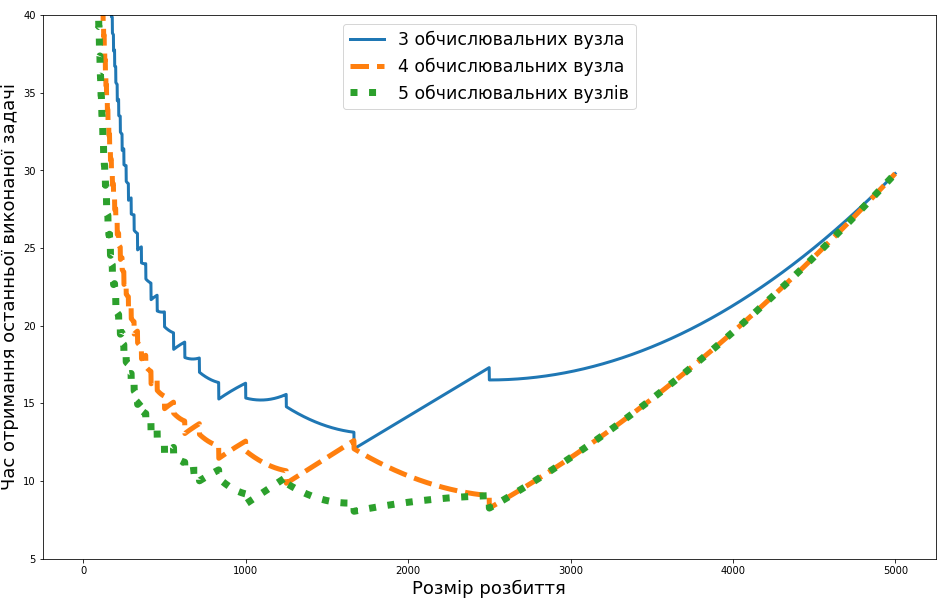
\includegraphics[width=\textwidth]{practice/img/one_user_different_proc}
	\caption{Графік залежності часу виконання всіх задач користувача від розміру розрізання для різних кількостей обчислювальних вузлів}
	\label{fig:one_diff_proc}
\end{figure}

На Рис. \ref{fig:one_diff_proc} зображено залежність часу симуляції від розбиття при фіксованих N, latency, bandwidth для 3, 4 та 5 обчислювальних вузлів. Чим більше ОВ, тим швидше множення матриць, проте для деяких розрізань можна побачити майже однаковий час при різній кількості обчислювальних вузлів. Особливо це помітно для 4 та 5, починаючи з розміру розрізання 2500 час для них однаковий хоч для обчислень і задіяно більше ОВ.

\begin{figure}[H]
	\centering
	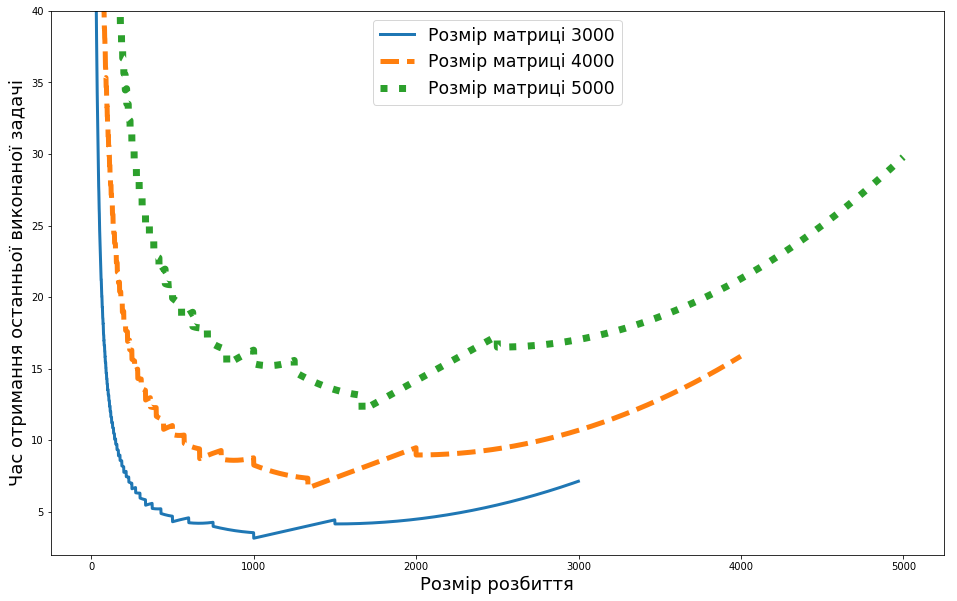
\includegraphics[width=\textwidth]{practice/img/one_user_different_N}
	\caption{Графік залежності часу виконання всіх задач користувача від розміру розрізання для різних розмірів матриць}
	\label{fig:one_diff_N}
\end{figure}

На Рис. \ref{fig:one_diff_N} показано для розмірів матриць 3000, 4000 та 5000 графіки залежності часу виконання усіх задач користувача від розбиття для 5 ОВ. З нього відносно можна помітити, що графіки мають приблизно однакову форму і можливо між ними має місце звичайна пропрорційну залежність від розміру матриці N.

\subsection{Симуляція для двої користувачів}

\begin{figure}[H]
	\centering
	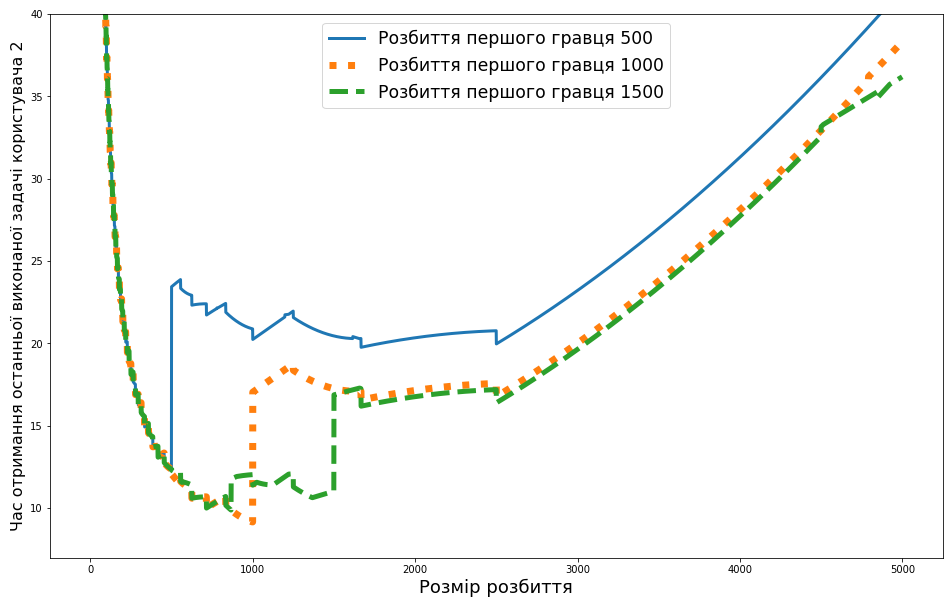
\includegraphics[width=\textwidth]{practice/img/two_users_fixed_first}
	\caption{Графік залежності часу виконання всіх задач другого користувача від розміру його стратегії розрізання при фіксованих стратегіях першого користувача}
	\label{fig:two_users_fixed_first}
\end{figure}

На Рис. \ref{fig:two_users_fixed_first} зображено залежність часу виконання усіх задач другого користувача від розміру розбиття при фіксованому розбитті користувача 1 для 5 ОВ. На графіку чітко спостерігається стрибки при переході розбиття користувача 2 за фіксоване значення розбиття користувача 1. Це особливість minmin та minmax оскільки вони в першу чергу виконують найлегші задачі, тому користувач, що вибрав менше розбиття, має менший час виконання усіх його задач.


\begin{figure}[H]
	\centering
	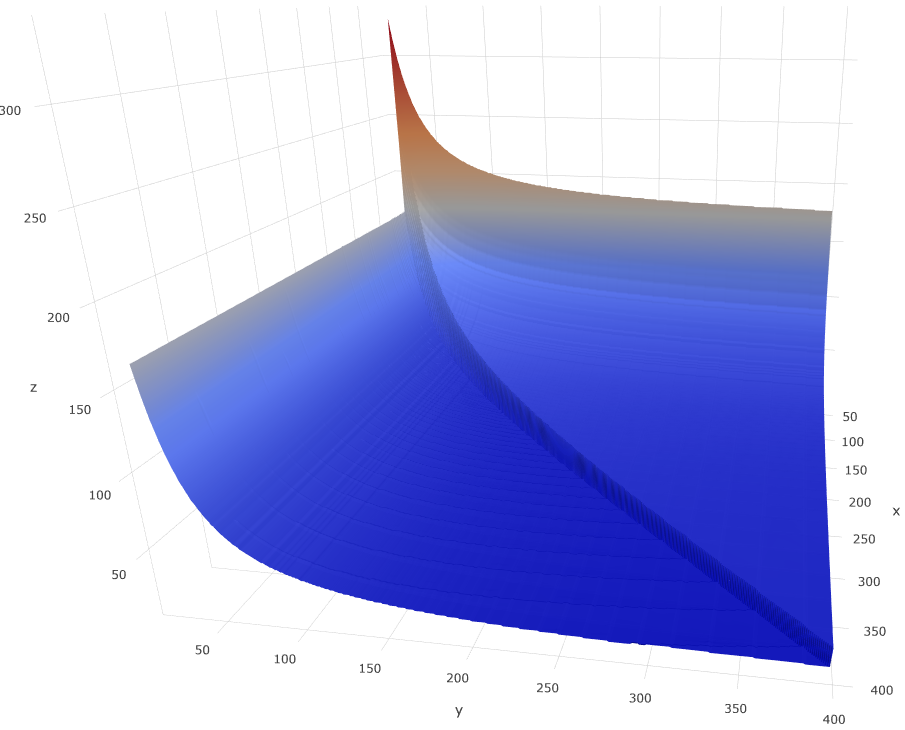
\includegraphics[width=\textwidth]{practice/img/two_users_surface_plot_20_400}
	\caption{Графік залежності часу виконання всіх задач другого користувача для всіх комбінацій стратегій обох користувачів з відрізка $[20, 400]$}
	\label{fig:two_users_surface_plot_20_400}
\end{figure}

На перший погляд поверхя, яка отримана шляхом симуляції усіх можливих пар стратегій обох користувачів з відріка $[20, 400]$, може здааватися гладкою та випуклою Рис. \ref{fig:two_users_surface_plot_20_400}. Проте, пам'ятаючи природу графіків при фіксованій стратегії першого користувача на Рис. \ref{fig:two_users_fixed_first}, слід подивитися на Рис. \ref{fig:two_users_surface_plot_20_400} більш ретельно, наприклад побудувати поверхню усіх комбінацій стратегій з відрізка $[150, 350]$.

\begin{figure}[H]
	\centering
	\begin{subfigure}[b]{0.45\textwidth}
		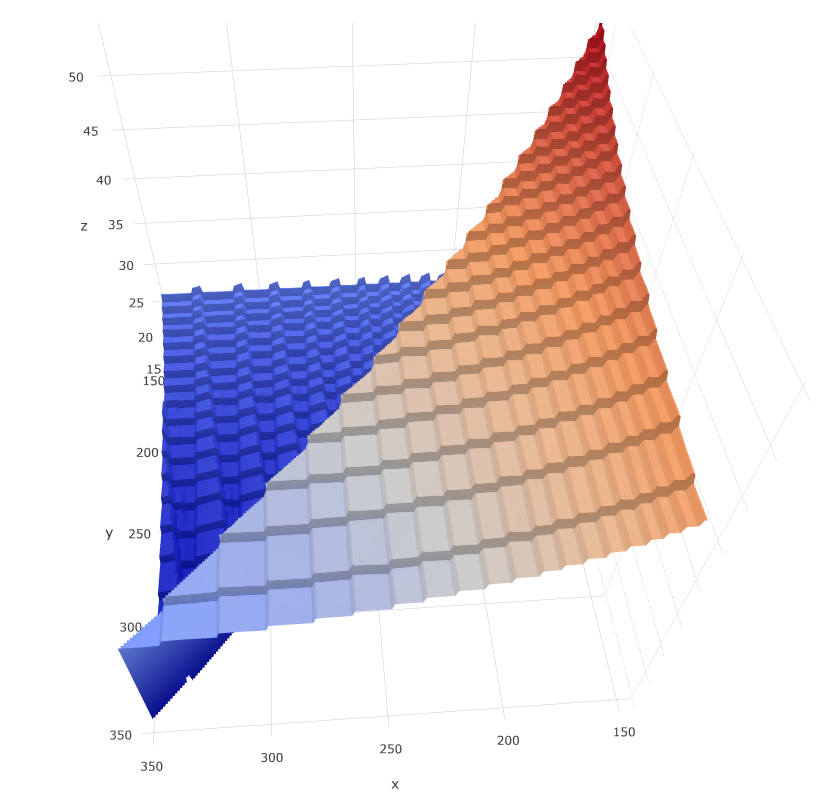
\includegraphics[width=\textwidth]{practice/img/two_users_surface_plot_150_350_top}
		\caption{Верхня частина графіка}
		\label{fig:two_users_surface_plot_150_350_top}
	\end{subfigure}
	\hfill
	\begin{subfigure}[b]{0.45\textwidth}
		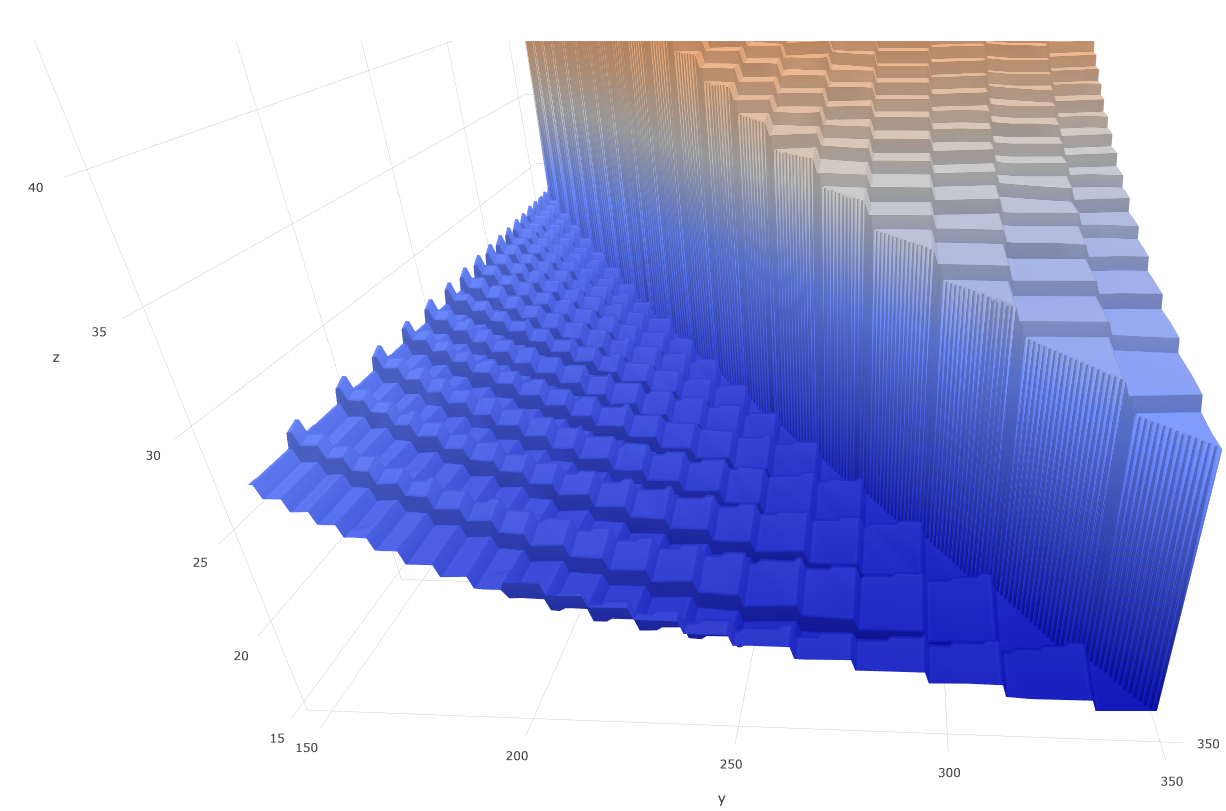
\includegraphics[width=\textwidth]{practice/img/two_users_surface_plot_150_350_bot}
		\caption{Нижня частина графіка}
		\label{fig:two_users_surface_plot_150_350_bot}
	\end{subfigure}
	\caption{Графік залежності часу виконання всіх задач другого користувача для всіх комбінацій стратегій обох користувачів з відрізка $[150, 350]$, \ref{fig:two_users_surface_plot_150_350_top} - фокус на верхню частину поверхні, \ref{fig:two_users_surface_plot_150_350_bot} - фокус на нижню частину поверхні}
	\label{fig:two_users_surface_plot_150_350}
\end{figure}

При кращій деталізації можна чітко побачити, що на Рис. \ref{fig:two_users_surface_plot_150_350_top} спостерігається форма сходинок по всій верхній частині графіка і вона не така проблемна, як нижня частина, показана на Рис. \ref{fig:two_users_surface_plot_150_350_bot}. Оскільки нижня частина більш цікава через те, що час завершення усіх задач користувача там менший, то і глобальний мінімум варто шукати саме на нижній частині. Нижня частина має особливої форми канави і саме вони є основною проблемою.





